\documentclass{beamer}
%
% Choose how your presentation looks.
%
% For more themes, color themes and font themes, see:
% http://deic.uab.es/~iblanes/beamer_gallery/index_by_theme.html
%
\mode<presentation>
{
  \usetheme{Madrid}      % or try Darmstadt, Madrid, Warsaw, ...
  \usecolortheme{beaver} % or try albatross, beaver, crane, ...
  \usefonttheme{serif}  % or try serif, structurebold, ...
  \setbeamertemplate{navigation symbols}{}
  \setbeamertemplate{caption}[numbered]
} 

\usepackage[english]{babel}
\usepackage[utf8x]{inputenc}
\usepackage{xcolor}
\usepackage{animate}

\usepackage{physics}
\usepackage{listings}
\lstset
{
    language=[LaTeX]TeX,
    breaklines=true,
    basicstyle=\tt\scriptsize,
    %commentstyle=\color{green}
    keywordstyle=\color{blue},
    %stringstyle=\color{black}
    identifierstyle=\color{magenta},
}

\title[University of Heidelberg]{Cosmological Evidences of Dark Matter from the Cosmic Microwave Background}
\author{Lorenzo Speri}
\date{November 2, 2018}

\AtBeginSection[]
{
  \begin{frame}<beamer>
    \frametitle{Outline}
    \tableofcontents[currentsection,currentsubsection]
  \end{frame}
}

\begin{document}

\begin{frame}
  \titlepage
\end{frame}

% Uncomment these lines for an automatically generated outline.
%\begin{frame}{Outline}
%  \tableofcontents
%\end{frame}

\section{Introduction}

\begin{frame}{Cosmic Microwave Background}
  


\begin{center}
\animategraphics[loop,controls,width=\textwidth]{1}{something-}{0}{3}\\
%\tiny
Accurate measurements of the temperature fluctuations of the CMB\\ help  us to understand the energy-matter content of our Universe

\end{center}
\end{frame}

\begin{frame}{The best Black Body Spectrum}
\begin{figure}
   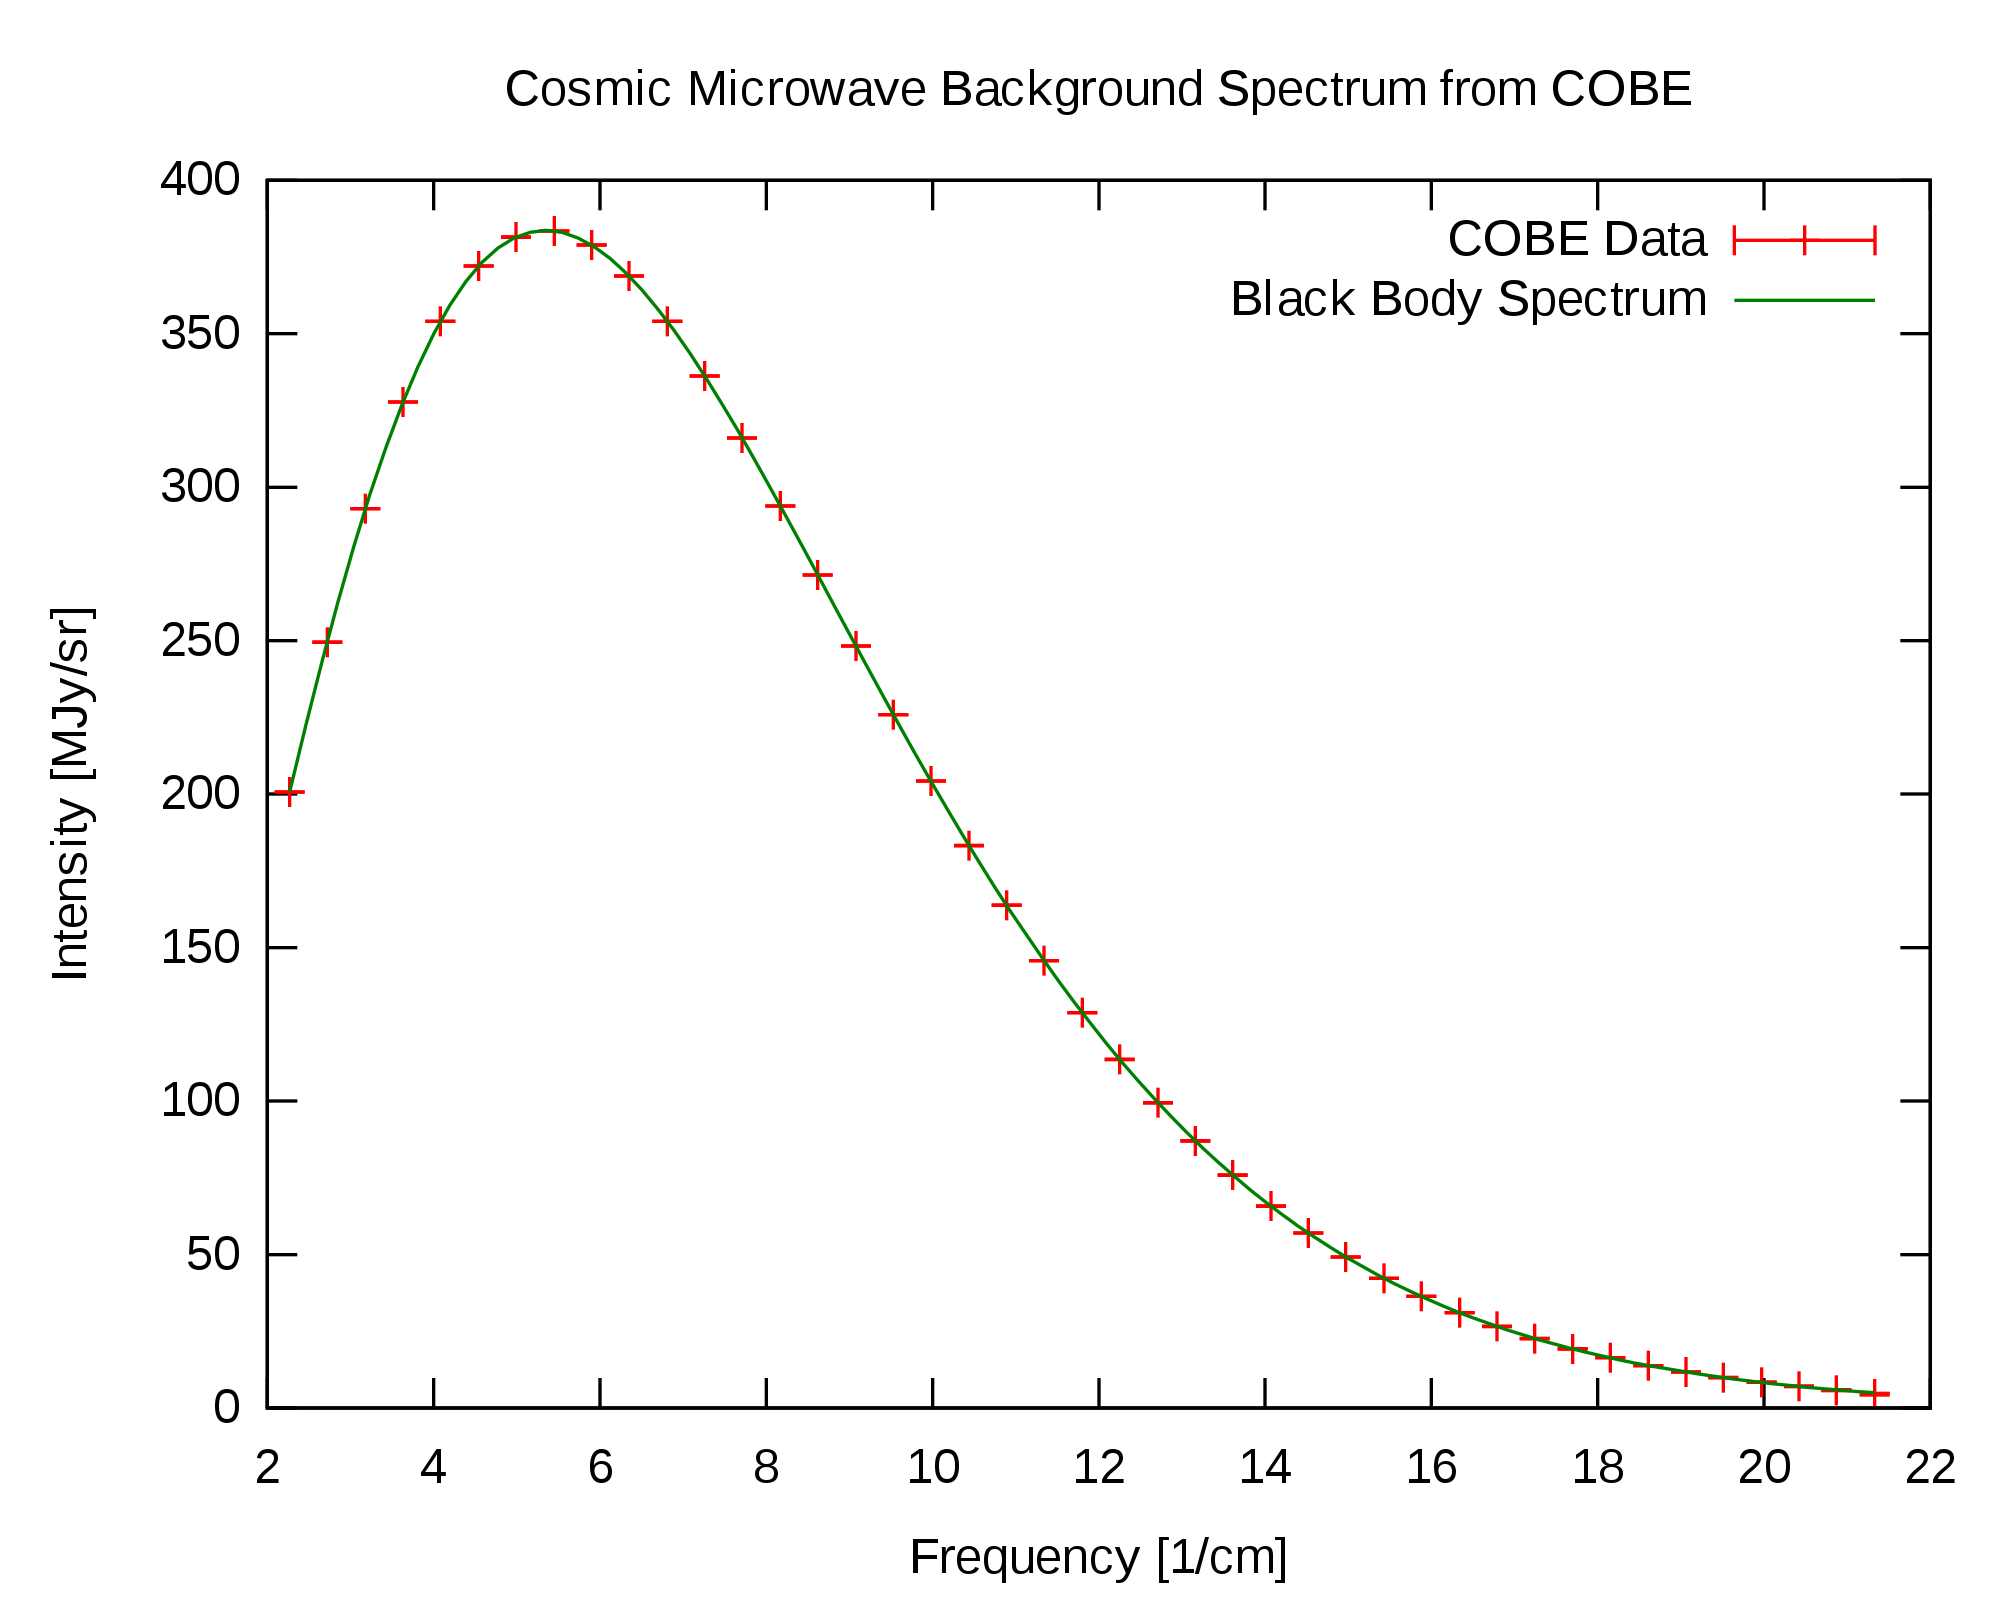
\includegraphics[height=6.5cm]{blackbody.png}
\end{figure}
$$<T_{CMB}> = 2.728 \pm 0.004 \text{ K}$$ 
\end{frame}

\begin{frame}{Dicrepancy between the expected temperature fluctuations}
At the decoupling time, the density contrast 
\[
\delta \rho = \frac{\rho - <\rho>}{<\rho>} \approx 10^{-3}
\]
If the CMB energy density $u$ were of equal magnitude, temperature fluctuations in the CMB should be of order $10^{-3}$ because
\[
u \propto T^4 \quad \Rightarrow \quad \frac{\delta u}{u} = 4 \frac{\delta T}{T}
\]
But the measured temperature fluctuations are of order $10^{-5}$ !
%It was realised later that the problem can be solved if dark matter does not electromagnetically interact, because then structures can form in the dark matter much before decoupling without leaving a direct imprint on the CMB temperature fluctuations. This is the strongest argument that dark matter should not interact electromagnetically, and probably only through the weak interaction.
\end{frame}


\section{$\Lambda$CDM model}
\begin{frame}{Assumptions of the $\Lambda$CDM model}

\begin{columns}
		\begin{column}{3cm}
			 \animategraphics[loop,controls,height=3cm]{4}{exp-}{0}{20}
			\begin{center}
				\tiny
				Spherical Harmonics
			\end{center}
		\end{column}
		\begin{column}{6cm}
			At 'enough' large scales $> 100$ Mpc, the Universe is
	\begin{itemize}
  		\item Homogeneous  
  		\item Isotropic
	\end{itemize}
		\end{column}
	\end{columns}
% class of observer that satisfies these assumption

	\vspace{0.5cm}
So the line element can be expressed as
\begin{equation*}
    \dd s^2 = g_{\mu \nu} \dd x^\mu \dd x^\nu = -c^2 \dd t^2 + a(t)^2 
    \qty( \frac{\dd r^2}{1-K r^2} + r^2 \dd \Omega ^2 )
\end{equation*}
where $a(t)$ is the scale factor and $K$ is the curvature of the Universe
\end{frame}

\begin{frame}{Friedmann Equations}
In addition, we trust Einstein's General Theory of Relativity
\begin{equation*}
    R^{\mu \nu} - \frac{1}{2}R g^{\mu \nu} + \Lambda g^{\mu \nu} = \frac{8 \pi G}{c^4} T^{\mu \nu}
\end{equation*}
\vspace{0.3cm}
Einstein’s field equations reduce to Friedmann’s equations
\begin{eqnarray}
     H^2 = \qty(\frac{\dot{a}}{a})^2 = \frac{8 \pi G \rho}{3} - \frac{K c^2}{a^2} + \frac{\Lambda  c^2}{3} \notag \\
\notag \\
     \dv{}{t}\qty{\rho c^2 a^3} + p \dv{}{t} \qty{a^3} =0 \notag
\end{eqnarray}
 where the Hubble constant is defined as $H_0 = H(t_0) = 100 h km s^{-1} Mpc^{-1} = $ and $h = 0.6727$
\end{frame}


\begin{frame}{Matter content \& Cosmic Rule}

    	\begin{columns}
        	\begin{column}{0.5\textwidth}
        	    	\begin{center}
        	    	Radiation $p = \frac{\rho c^2}{3}$
        	    	$$\rho = \rho_0 a^{-4}$$
              	\end{center}

        	\end{column}
            \begin{column}{0.5\textwidth}
             \begin{center}
              Dust $p=\rho \ll \rho c^2$
              $$\rho = \rho_0 a^{-3}$$
             \end{center}
        	\end{column}
    	\end{columns}
    	
    	\vspace{0.5cm}
    	Friedmann's equations can be rewritten using:
    	\begin{eqnarray}
    	     \Omega_R = \frac{8 \pi G \rho_R}{3 H_0 ^2} \qquad
    	     \Omega_M =  \frac{8 \pi G \rho_M}{3 H_0 ^2} \qquad
    	     \Omega_\Lambda =  \frac{\Lambda}{3 H_0 ^2} \qquad
    	     \Omega_K = -\frac{K}{a_0 ^2 H_0 ^2} \notag
    	\end{eqnarray}
    	    	
    	$$
    	H^2 = H_0 ^2 \qty{\Omega_R \frac{a_0 ^4}{a^4} + \Omega_M \frac{a_0 ^3}{a^3} + \Omega_\Lambda + \Omega_K \frac{a_0 ^2}{a^2}} 
    	$$
    	At $a =a_0$ $\Rightarrow$ today, we get the Cosmic Rule: 
    	$$
    	1 = \Omega_R +  \Omega_M + \Omega_\Lambda + \Omega_K
    	$$
    	\end{frame}

\begin{frame}{Multipoles Decomposition}
    	\begin{columns}
		\begin{column}{4cm}
			 \animategraphics[loop,controls,width=\textwidth]{4}{multipole-}{0}{34}
			\begin{center}
				\tiny
				Spherical Harmonics
			\end{center}
		\end{column}
		\begin{column}{6cm}
			Projection of the temperature fluctuations onto another set of basis functions which are orthonormal on the sky:
			$$
			 T(\theta,\phi) = \sum_{l,m} a_{lm} Y^m _l (\theta,\phi)
			$$
			
			And $$C_l = \frac{1}{2l +1} \sum _{m=-l} ^l \abs{a_{lm}} ^2$$
		\end{column}
	\end{columns}
    
\end{frame}

\begin{frame}{Temperature Power Spectrum Planck 2015}
    \begin{figure}
   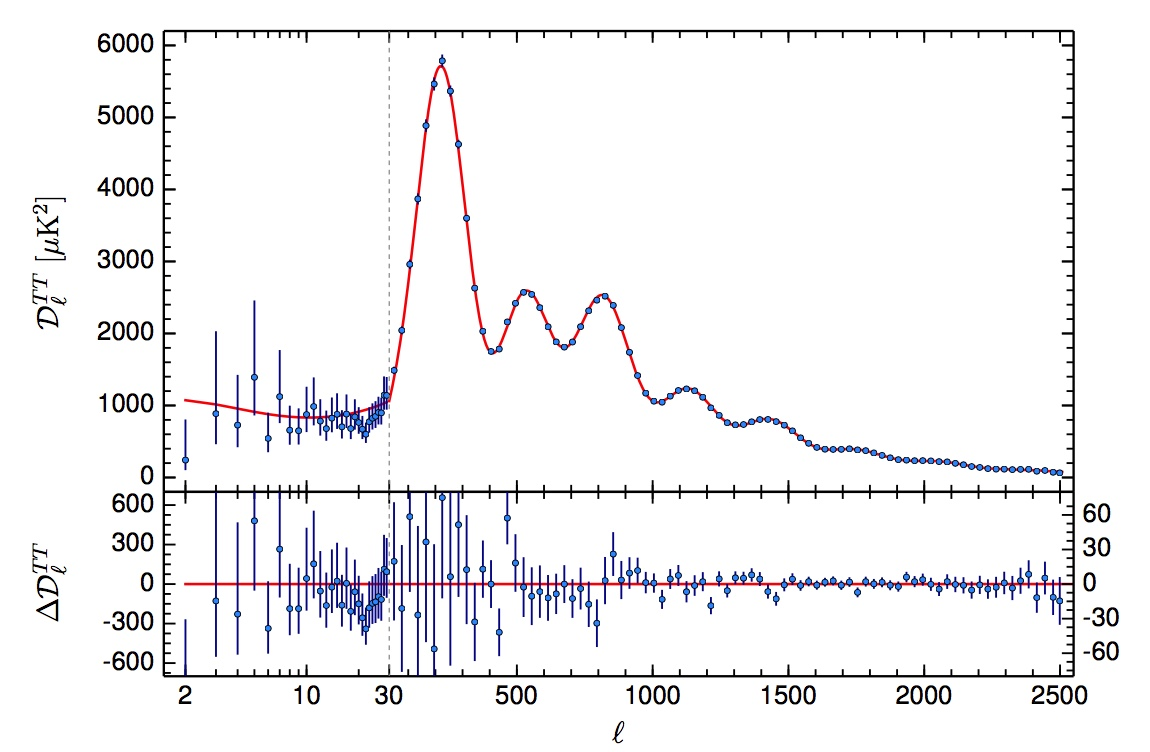
\includegraphics[height=7cm]{planck2015.jpeg}
\end{figure}
$$D_l ^{TT} = l(l+1)C_l/(2\pi)$$
\end{frame}

\begin{frame}{Temperature Power Spectrum and Angular size}
    \animategraphics[loop,controls,width=\textwidth]{2}{filter-}{0}{18}\\
    \begin{center}
        For large $l$, $
			\theta \sim 1/l
			$
    \end{center}
    
\end{frame}


\section{The role of the Dark Matter}

\begin{frame}{Variations of the cosmological parameters}
% we can see where the dark matter played an important role
    \begin{figure}
   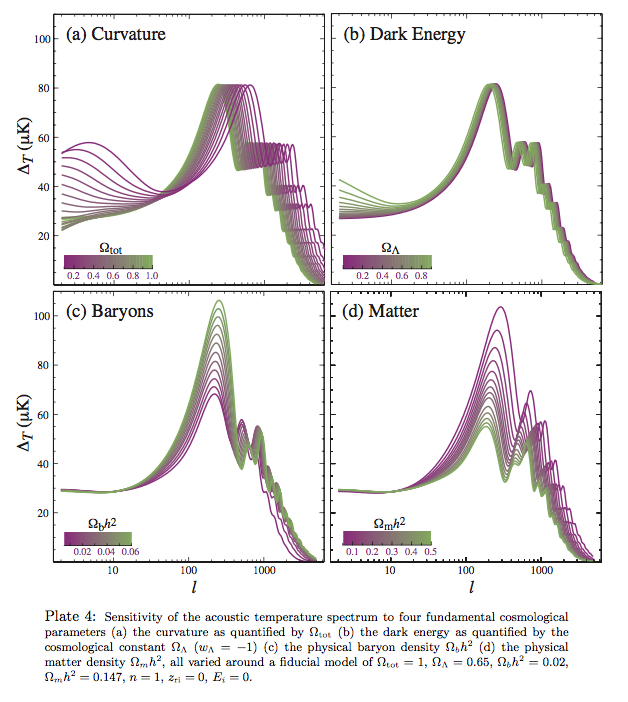
\includegraphics[height=8cm]{dt_parameter_variation}
\end{figure}

\end{frame}

\begin{frame}{Variations of the Dark Matter density}
\begin{columns}
  \begin{column}{6cm}
   \animategraphics[loop,controls,height=6cm]{10}{matter_change-}{0}{27}
\end{column}
		\begin{column}{4cm}
		\begin{itemize}
		    \item Raising the dark matter density reduces the overall amplitude of the peaks
		    \item  High third peak is an indication of dark matter
		\end{itemize}

\end{column}
	\end{columns}
\end{frame}

\begin{frame}{Variations of the Baryon density}
% we can see where the dark matter played an important role
  \begin{center}
  
  \begin{columns}
		\begin{column}{6cm}
			 \animategraphics[loop,controls,height=6cm]{10}{baryon_change-}{0}{19}
		\end{column}
		\begin{column}{4cm}
			\begin{itemize}
			\small
			    \item Power spectrum shows baryons enhance every other peak
			    %The odd numbered acoustic peaks are enhanced in amplitude over the even numbered ones as $\Omega_B h^2$ increases
			    \item  Second peak is suppressed compared with the first and third
			    %since adding mass to a spring slows the oscillation down, adding baryons to the plasma decrease the frequency of the oscillations pushing the position of the peaks to slightly higher multipoles l
			    \item Adding baryons to the plasma decrease the frequency of the oscillations pushing the position of the peaks to slightly higher multipoles l
			\end{itemize}
		\end{column}
	\end{columns}
   
\end{center}
\end{frame}


\begin{frame}{Acoustic Oscillations}
At the time before recombination:
\begin{itemize}
    \item Dark Matter is randomly distributed
    \item if a portion of photon-baryon fluid is in a potential well of the dark matter, it will fall to the center of the well
    \item gravity compresses the photon-baryon fluid
    \item pressure starts to rise
    \item the pressure is sufficient to cause the fluid to expand outward
    \item the pressure drops until gravity causes the photon-baryon fluid to fall inward again
\end{itemize}
\begin{center}
    \animategraphics[loop,controls,height=3cm]{10}{plane-}{0}{7}

\end{center}
\end{frame}



\begin{frame}{Acoustic Oscillations: Simple Model}


		
			\animategraphics[loop,controls,width=\textwidth]{5}{hotcold-}{0}{9}
		
		
			\begin{itemize}
			    \item Quantum fluctuations from the early universe generates both density enhancements and deficits
			    \item During the inflation these quantum fluctuations had been stretched into cosmic scales
			\end{itemize}




\end{frame}


\begin{frame}{Parameters from Planck 2015}
CMB \& temperature power spectrum  $+$ nucleosynthesis analysis $\Rightarrow$ Dark-matter density.
\vspace{0.3cm}
\begin{itemize}
    \item Dark-matter density $0.2647$ $\Rightarrow$ relative error $1.6 \%$
    \vspace{0.3cm}
    \item Dark-energy density $0.6844$ $\Rightarrow$ relative error $1.3 \%$
        \vspace{0.3cm}

    \item Baryonic matter density $0.04917$ $\Rightarrow$ relative error $1.2 \%$
        \vspace{0.3cm}

    \item Radiation density $8.51 \times 10^{-5}$ $\Rightarrow$ relative error $0.6 \%$
\end{itemize}
     %\begin{figure}
   %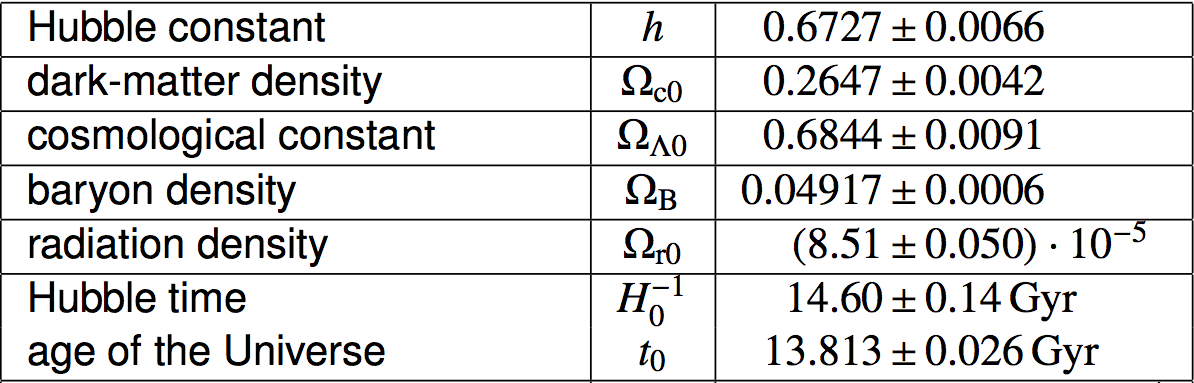
\includegraphics[width=10cm]{table.jpg}
%\end{figure}
\end{frame}

\begin{frame}{Dark Matter matters ... for anisotropies!}
    \begin{itemize}
        \item Dark Matter interacts with the photons and matter through the gravitational potentials causing fluctuations.
        \vspace{0.5cm}
        \item Fluctuations are  responsible for anisotropy formations
        \vspace{0.5cm}
        \item The resultant fluctuations appear to the observer today as anisotropies on the sky
    \end{itemize}

\end{frame}



\begin{frame}[allowframebreaks]{References}
\nocite{*}
\bibliographystyle{plain}
\bibliography{dark_bib.bib}
\end{frame}



\end{document}
